\documentclass{article}
\usepackage[utf8]{inputenc}
\usepackage{graphicx} % Required for inserting images
\usepackage{hyperref}
\usepackage{subcaption}
\usepackage{float}
\usepackage{tcolorbox}
\usepackage{amsmath}
\usepackage{amssymb}
\usepackage{listings}% http://ctan.org/pkg/listings}
\usepackage{algorithm}
\usepackage{algorithmic}
\usepackage[toc,page]{appendix}
\usepackage[backend=biber]{biblatex}
\usepackage{multicol}
\usepackage{siunitx}
\usepackage{comment}
\usepackage{xcolor}
\usepackage{caption}
\usepackage{tikz}
\usetikzlibrary{shapes.geometric, arrows}

\tikzstyle{startstop} = [rectangle, rounded corners, 
minimum width=3cm, 
minimum height=1cm,
text centered, 
draw=black, 
fill=red!30]

\tikzstyle{io} = [trapezium, 
trapezium stretches=true, % A later addition
trapezium left angle=70, 
trapezium right angle=110, 
minimum width=3cm, 
minimum height=1cm, text centered, 
draw=black, fill=blue!30]

\tikzstyle{process} = [rectangle, 
minimum width=3cm, 
minimum height=1cm, 
text centered, 
text width=3cm, 
draw=black, 
fill=orange!30]

\tikzstyle{decision} = [diamond, 
minimum width=3cm, 
minimum height=1cm, 
text centered, 
draw=black, 
fill=green!30]
\tikzstyle{arrow} = [thick,->,>=stealth]

% To delete lstlisting caption "Listing x"
%\captionsetup[lstlisting]{labelformat=empty}

\lstdefinestyle{myStyle}{
    belowcaptionskip=1\baselineskip,
    breaklines=true,
    frame=none,
    numbers=none, 
    basicstyle=\footnotesize\ttfamily,
    keywordstyle=\bfseries\color{green!40!black},
    commentstyle=\itshape\color{purple!40!black},
    identifierstyle=\color{black},
    backgroundcolor=\color{white},
}

\lstdefinestyle{cypherStyle}{
    backgroundcolor=\color{white},   % choose the background color
    basicstyle=\footnotesize\ttfamily,        % the size of the fonts that are used for the code
    commentstyle=\itshape\color{purple!40!black},
    keywordstyle=\bfseries\color{green!40!black},
    breakatwhitespace=false,         % sets if automatic breaks should only happen at whitespace
    breaklines=true,                 % sets automatic line breaking
    captionpos=b,                    % sets the caption-position to bottom
    commentstyle=\color{gray},    % comment style
    deletekeywords={},            % if you want to delete keywords from the given language
    escapeinside={\%*}{*)},          % if you want to add LaTeX within your code
    extendedchars=true,              % lets you use non-ASCII characters; for 8-bits encodings only, does not work with UTF-8
    %firstnumber=1000,                % start line enumeration with line 1000
    frame=none,                    % adds a frame around the code
    keepspaces=true,                 % keeps spaces in text, useful for keeping indentation of code (possibly needs columns=flexible)
    language=SQL,                    % the language of the code
    morekeywords={*,IF, REQUIRE, FOR, IS, LOAD, CSV, WITH, HEADERS, MERGE, toFloat, toInteger, date},            % if you want to add more keywords to the set
    numbers=none,                    % where to put the line-numbers; possible values are (none, left, right)
    numbersep=5pt,                   % how far the line-numbers are from the code
    numberstyle=\tiny\color{mygray}, % the style that is used for the line-numbers
    rulecolor=\color{black},         % if not set, the frame-color may be changed on line-breaks within not-black text (e.g. comments (green here))
    showspaces=false,                % show spaces everywhere adding particular underscores; it overrides 'showstringspaces'
    showstringspaces=false,          % underline spaces within strings only
    showtabs=false,                  % show tabs within strings adding particular underscores
    stepnumber=1,                    % the step between two line-numbers. If it's 1, each line will be numbered
    stringstyle=\ttfamily,     % string literal style
    tabsize=2,                       % sets default tabsize to 2 spaces
}

%% Golang definition for listings
%% http://github.io/julienc91/lstlistings-golang
%%
\lstdefinelanguage{Golang}%
  {morekeywords=[1]{package,import,func,type,struct,return,defer,panic,%
     recover,select,var,const,iota,},%
   morekeywords=[2]{string,uint,uint8,uint16,uint32,uint64,int,int8,int16,%
     int32,int64,bool,float32,float64,complex64,complex128,byte,rune,uintptr,%
     error,interface},%
   morekeywords=[3]{map,slice,make,new,nil,len,cap,copy,close,true,false,%
     delete,append,real,imag,complex,chan,},%
   morekeywords=[4]{for,break,continue,range,go,goto,switch,case,fallthrough,if,%
     else,default,},%
   morekeywords=[5]{Println,Printf,Error,Print,},%
   sensitive=true,%
   morecomment=[l]{//},%
   morecomment=[s]{/*}{*/},%
   morestring=[b]',%
   morestring=[b]",%
   morestring=[s]{`}{`},%
}

\lstdefinestyle{golangStyle}{
    captionpos=b,              % sets the caption-position to bottom
    belowcaptionskip=1\baselineskip,
    breaklines=true,
    frame=none,
    numbers=none, 
    basicstyle=\footnotesize\ttfamily,
    keywordstyle=\bfseries\color{green!40!black},
    commentstyle=\itshape\color{purple!40!black},
    identifierstyle=\color{black},
    backgroundcolor=\color{white},
    language=Golang,
}


\title{TFM-FernandoMartín}
\author{Fernando Martín Canfrán}
\date{April 2024}

\begin{document}

\section{Synthetic dataset creation}

Given the confidential and private nature of bank data, it was not possible to find
any real bank datasets to perform our experiments on. In this regard, a synthetic property
graph bank dataset was built based on the Wisabi Bank Dataset\footnote{\href{https://www.kaggle.com/datasets/obinnaiheanachor/wisabi-bank-dataset}{Wisabi bank dataset on kaggle}}. It is a fictional banking dataset that 
was designed and architected by Obinna Iheanachor, and that was made publicly available in
the Kaggle platform.
 

In particular it contains 10 CSV tables. Five of them are of transaction records of five 
different states of Nigeria (Federal Capital Territory, Lagos, Kano, Enugu and Rivers State) 
that refers to transactions of cardholders in ATMs. In particular they contain 2143838 
transactions records done during the year 2022, of which 350251 are in Enugu, 159652 in 
Federal Capital Territory, 458764 in Kano, 755073 in Lagos and 420098 in Rivers.

Then, the rest of the tables are: a customers table (`customers\_lookup`) where the data
of 8819 different cardholders is gathered, an ATM table (`atm\_location lookup`) with
information of each of the 50 different locations of the ATMs, and then three remaining
tables as complement of the previous ones (`calendar lookup`, `hour lookup` and 
`transaction\_type lookup`) 
(\href{https://app.diagrams.net/#G1eAn47YR7-zPNE5KgStkA6_IJcxZRYgX8#%7B%22pageId%22%3A%22R2lEEEUBdFMjLlhIrx00%22%7D}{tables summary}).

Based on the aforementioned dataset we created our own synthetic dataset. For simplicity 
and to do it in a more stepwise manner, we are going to first create all the CSV data tables
for the nodes and for the relations in the corresponding format and then we will populate 
the Neo4j GDB with those.
The description of the creation of the CSV data tables as well as the specific details are 
described in what follows:

\subsubsection*{Bank}

\begin{tcolorbox}
\textcolor{red}{$\Rightarrow$ Only 1 bank}
\end{tcolorbox}

\begin{itemize}
\item[-] name: Bank name.
\item[-] code: Bank identifier code.
\item[-] loc\_latitude: Bank headquarters GPS-location latitude.
\item[-] loc\_longitude: Bank headquarters GPS-location longitude.
\end{itemize} 

The generation of the Banks is done taylored to our needs as we are only considering a 
reduced amount of Bank entities. In particular we generated three different Banks. 
\texttt{n} ATMs and \texttt{m} Cards belonging to each of them, will be generated as 
explained in what follows. Note that apart from the generation of the entities ATM and 
Card we will also need to generate the relationships ATM-Bank (\texttt{belongs\_to}) and 
Card-Bank (\texttt{issued\_by}) that matches each of these entities with the corresponding 
Bank entity to which they belong. 

\subsubsection*{ATM}

\begin{itemize}
\item[-] ATM\_id: Unique identifier of the ATM.
\item[-] loc\_latitude: GPS-location latitude where the ATM is located.
\item[-] loc\_longitude: GPS-location longitude where the ATM is located.
\item[-] city: City in which the ATM is located.
\item[-] country: Country in which the ATM is located.
\end{itemize}

The generation of \texttt{n} ATMs for the bank is done following
the geographical distribution of the locations of the ATMs in the wisabi dataset. On it there are 50 ATMs
locations distributed along Nigerian cities. The distribution of the ATMs matches the
importance of the location since the number of ATM locations is larger in the most populated 
Nigerian cities (30\% of the ATM locations are in the city of Lagos, then the 20\% in 
Kano...) Therefore, for generating a new ATM location first we select uniformly at 
random an ATM location/city from the wisabi dataset, which is directly assigned as 
\texttt{city} and \texttt{country} to the ATM instance, and generate new random 
geolocation coordinates inside a constructed bounding box of this city location to set 
as the \texttt{loc\_latitude} and \texttt{loc\_longitude} of the ATM.

\begin{tcolorbox}
\textcolor{red}{$\Rightarrow$ Okay like this: }
\textcolor{blue}{Note that we do not take into account for the density distribution of the 
ATMs of the wisabi dataset that, for each ATM location of the dataset, we have \texttt{x} 
number of atms.}

Aspects to explain:
\begin{itemize}
  \item Geographical distribution of the ATMs based on the geographical distribution 
  of the locations of the Wisabi ATMs.
  \item Do a plot of the geographical dist of the positions of the ATMs of the wisabi dataset.
\end{itemize}
\end{tcolorbox}

\subsubsection*{Card}

\begin{itemize}
\item[-] number\_id: Unique identifier of the card.
\item[-] client\_id: Unique identifier of the client.
\item[-] expiration: Validity expiration date of the card.
\item[-] CVC: Card Verification Code.
\item[-] extract\_limit: Limit amount of money extraction associated with the card.
\item[-] loc\_latitude: Client address GPS-location latitude.
\item[-] loc\_longitude: Client address GPS-location longitude.
\end{itemize}

\begin{tcolorbox}
  Aspects to explain:
  \begin{itemize}
    \item Extended behavior fields: to not only withdrawal.
    \item Location: Explain the 2 options we have developed and the one used so far.
    \item Explain how the behavior of the card is generated based on a random
    selected wisabi customer.
    \item Extract\_limit: explain how and why?
  \end{itemize}
\end{tcolorbox}

For the Card entity generation there are some different aspects that are worth to mention:
\begin{itemize}
    \begin{tcolorbox}
      \item First, in relation with the card and client identifiers (\texttt{number\_id}, 
      \texttt{client\_id}), \textcolor{blue}{for the moment we define that each client has 
      1 card, later this can be modified.\\}
      \textcolor{red}{$\Rightarrow$ For the moment 1 client : 1 card. So far, 
      for the kind of frauds we are considering this is the easier approach. In a 
      future, if needed, it could be generated the case that 1 client has n cards} 
    \end{tcolorbox}

    \item \texttt{Expiration} and \texttt{CVC} fields: they are not relevant, could be empty 
    fields indeed or for all the Cards the same values. For simplicity and completeness we 
    chose them to be the same values for all the Cards.
    \begin{tcolorbox}
      Expiration: set for completeness the same date in all of them but in a far future!
    \end{tcolorbox}
    \item \textcolor{blue}{Behavior: For each Card object to be generated, we assign it a 
    \textit{behavior} based on the transaction behavior of a randomly selected wisabi 
    customer. The behavior is gathered from the transaction history of the customer on 
    the wisabi dataset. This will be particularly useful later for the generation of the 
    synthetic transactions, so that for each of the cards their transactions can be 
    simulated based on this gathered behavior.}
    In particular the customer \textit{behavior} refers to: 
    \begin{itemize}
        \item \texttt{extract\_limit}: maximum normal amount that a card can extract. 
        $\textcolor{blue}{\texttt{amount\_avg} * 5}$.
        \item \texttt{amount\_avg}: extracted amount average of the customer on a transaction.
        \item \texttt{amount\_std}: extracted amount standard deviation of the customer 
        on a transaction.
        \item \texttt{withdrawal\_day}: average number of transactions per day of the 
        customer. \textcolor{red}{Withdrawals only for the moment!}.
    \end{itemize}
    \begin{tcolorbox}
      \item New added behavior: interesting for the generation of transactions that are
      not only withdrawals: balance inquiries, deposits, transfers.
    \end{tcolorbox}
    Note that all this fields are additionally added to the Card CSV records.
    Some additional remarks:
    \begin{itemize}
        \item \textcolor{red}{For the moment we only consider the \textit{withdrawal} type of transaction in the behavior. However \textit{transfer} and \textit{deposit} could be also considered.}
        % retirada de dinero 
        \item \textcolor{red}{This behavior is gathered from one random customer of the wisabi dataset per each of the Cards, so that we have more variability. However, we could also assign the same behavior to all the clients, and this behavior be like a summary of all the wisabi dataset clients behavior. Also the behavior could be assigned drawning it from taylored distributions selected by us, in a more customizable manner.}   
    \end{itemize}
    \item Location (\texttt{loc\_latitude}, \texttt{loc\_longitude}): Two possible options in this case:
    \begin{itemize}
        \item 1. Assign a random location of the usual ATM city/location of the random selected wisabi customer. This way, we maintain the geographical distribution of the wisabi customers.
        \item 2. Assign a random location of the city/location of a random ATM of the newly generated ATMs objects. (* For the moment)
    \end{itemize}
\end{itemize}

\subsubsection*{Transaction}

\begin{itemize}
\item[-] transaction\_id: Unique identifier for each transaction in the database.
\item[+] number\_id: Identifier of the card linked with the transaction.
\item[+] ATM\_id: Identifier of the ATM in which the transaction takes place.
\item[-] transaction\_start: Datetime when the transaction started. Format: DD/MM/YYYY HH:MM (ex. 1/1/2022 4:50).
\item[-] transaction\_end: Datetime when the transaction was completed. Format: DD/MM/YYYY HH:MM (ex. 1/1/2022 4:54).
\item[-] transaction\_amount: Amount of money involved in the transaction.
\end{itemize}


\begin{comment}
\textcolor{blue}{The transaction generator is done to be able to generate transactions for each of the cards based on the gathered client transaction behavior of each of the cards for a customisable \textcolor{orange}{\texttt{d}} number of days starting in a \textcolor{orange}{\texttt{start\_date}}. For a card, the idea is to create a certain number of transactions per day, by linking the card to a certain ATM that is no farther than \textcolor{orange}{\texttt{max\_distance}} kms from the residence location of the client of the card. Also, we will limit the time distance between two consecutive transactions so that the final set of created transactions can not produce a potential fraud related with having two transactions in different ATM locations with an insufficient feasible time distance.}
For each card:
\begin{itemize}
    \item ATM subset: Create a subset of ATMs that are considered to be \textit{usual} for the card client, so that they are all at a distance inferior or equal to \textcolor{orange}{\texttt{max\_distance}} kms to the residence location of the client of the card. We limit the size of this subset to be of \textcolor{orange}{\texttt{max\_size\_atm\_subset}}, so that we take only a maximum of \textcolor{orange}{\texttt{max\_size\_atm\_subset}} of the closest ATMs.
    \textcolor{blue}{In addition, among the ATMs in this subset, preference is given to those that are the closest to the residence location of the client and those that belong to the same bank company as the client's card.}
    The transactions generated for this card will be linked only to ATMs of this subset.
    \item \textcolor{orange}{\texttt{t\_min}}: Minimum threshold time in between two transactions of this client. That is, the minimum time distance between the end of a transaction and the start of the next consecutive transaction of a card. There are two options for the calculation of this minimum time distance:
    \begin{itemize}
        \item In general: taking $2*\texttt{max\_distance}$ kms as the upper bound on the maximum distance between 2 ATMs of the ATM subset, set the \textcolor{orange}{\texttt{t\_min}} to be the time needed to traverse that distance at 50km/h. (*: for the moment)
        \item Specifically: Taking the specific maximum distance between all the ATM pairs in the ATM subset to get the \textcolor{orange}{\texttt{t\_min}}.
    \end{itemize}  
    \item For each day generate \textcolor{orange}{\texttt{num\_tx}} transactions, random number drawn from a Poisson distribution of $\lambda = \texttt{withdrawal\_day}$.
    \item \textcolor{blue}{Distribution of the \texttt{num\_tx} transaction times (\texttt{transaction\_start}) during a day: we create an ordered list of \texttt{num\_tx} start moments in seconds in a day (in the range $[\texttt{t\_min}/2, 86400-(\texttt{t\_min}/2)-\texttt{max\_duration}]$) so that all of them are at a minimum time distance of $\texttt{t\_min} + \texttt{max\_duration}$. See Figure \ref{img:tx-distribution}.
    \textit{\texttt{max\_duration} limits the maximum duration of an ordinary transaction. For the moment it was set to be of 10 minutes (600s)}.\\
    Note that the interval bounds for the transaction start moments are designed in such a way that the \texttt{t\_min} minimum time distance between the end of a transaction and the start of the next transaction is also respected between transactions belonging to different consecutive days.} See Figure \ref{img:tx-distribution-day}. \textcolor{red}{Note that this way of generation (day by day) we are not allowing transactions to occur in the interval marked among the two red dotted lines of the Figure \ref{img:tx-distribution-day}.} \textcolor{orange}{NOTE/TODO: This could be fixed by looking to the start time of the last transaction of the previous day...}. 
    The start moments are therefore taken to define the \texttt{transaction\_start} of each of the transactions of that day. \texttt{transaction\_end} is assigned a shifted time difference with the respective \texttt{transaction\_start}, in particular the difference is drawn from a normal distribution $\mathcal{N}(300,\,120)$ that defines the duration of a transaction to be of mean of 5 minutes (300s) and a standard deviation of 2 minutes (120s), bounding it to be of a maximum time of \texttt{max\_duration} of 10 minutes (600s) and setting it to the mean if the distribution sample was negative. 
    \begin{figure}[H]
        \centering
        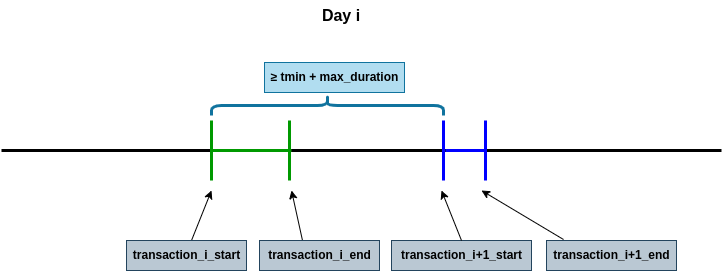
\includegraphics[scale = 0.45]{images/Synthetic-dataset-creation/tx-distribution-1.png}
        \caption{Time distance limit between two consecutive transactions}
        \label{img:tx-distribution}
    \end{figure}
    \begin{figure}[H]
        \centering
        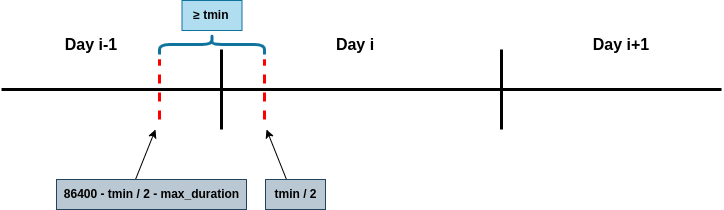
\includegraphics[scale = 0.45]{images/Synthetic-dataset-creation/tx-distribution.png}
        \caption{Time distance limit between two consecutive transactions between two days}
        \label{img:tx-distribution-day}
    \end{figure}
    Note that a limit was set on the duration of the transaction so that we can have the control avoiding time overlapping transactions, which will be producing irregular undesired fraud pattern alerts.
    \item \texttt{transaction\_amount}: based on card behavior parameters, it is drawn from a normal distribution 
    $\mathcal{N}(\texttt{amount\_avg},\,\texttt{amount\_std})$. If negative amount, drawn from a uniform distribution $\mathcal{U}(0,\ \texttt{amount\_avg}*2)$.
\end{itemize}

% --------------------------------------------------------------------------------------------------------------
% TODO: CONTINUE HERE 
Note that this approach is done with the focus on... taking into account the previous generated transaction: both for the linked ATM of the new transaction and its transaction time (to avoid transactions that are overlapped or that come one directly after the other --> this may be fraudulent - AVOID!) 
\end{comment}

\end{document}